\setcounter{chapter}{6}

\addcontentsline{toc}{section}{Homework 6}
\section*{Homework 6}

\begin{enumerate}
    \item \textit{Either give an example, or show that no such example exists.}
    
    A bounded function $h$ on $[0,3]$ such that for every partition $P$ of $[0,3]$, $U(h,P) = 5$ and $L(h,P) = 1$

    \begin{proof}[Solution]
        Consider: $h(x) = \begin{cases}
        \frac{5}{3}, & x \in \mathbb{Q} \\
        \frac{1}{3}, & x \notin \mathbb{Q}
        \end{cases}$

        \begin{center}
        \begin{tikzpicture}
            \begin{axis}[
                axis lines=middle,
                xlabel={$x$},
                ylabel={$y$},
                xmin=-0.5, xmax=3.5,
                ymin=0, ymax=2,
                xtick={0,1,2,3},
                ytick={1/3,5/3},
                yticklabels={$\frac{1}{3}$,$\frac{5}{3}$},
                width=10cm,
                height=6cm
            ]
            \addplot[domain=0:3, samples=2, very thick, blue] {1/3};
            \addplot[domain=0:3, samples=2, thin, red] {5/3};
            \end{axis}
        \end{tikzpicture}
        \end{center}

        $h$ is bounded by TREE(3).
        For all partitions, the upper sum is $5$ and the lower sum is $1$.
    \end{proof}

    A function $g$ on $[0,1]$ and partitions $P$ and $Q$ of $[0,1]$ where $U(g,P) = L(g,P)$ but $U(g,Q) \neq L(g,Q)$.
    
    \begin{proof}[Solution]
        Consider the function $g(x) = x$ on $[0,1]$.

            Let $P = \{0, 1\}$ and $Q = \{0, \frac{1}{2}, 1\}$.

            For partition $P$, the upper sum $U(g,P) = L(g,P) = \frac{1}{2}$.

            For partition $Q$, the upper sum $U(g,Q) \neq L(g,Q)$.

            \begin{center}
            \begin{tabular}{cc}
            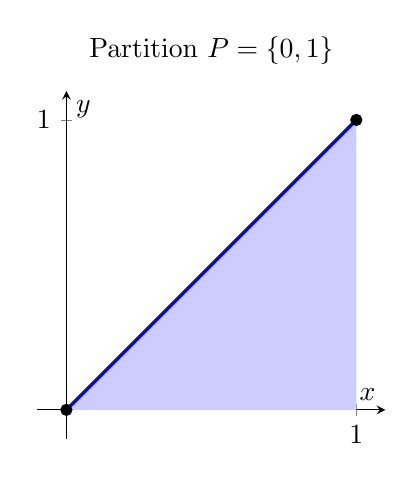
\begin{tikzpicture}
                \begin{axis}[
                axis lines=middle,
                xlabel={$x$},
                ylabel={$y$},
                xmin=-0.1, xmax=1.1,
                ymin=-0.1, ymax=1.1,
                xtick={0,1},
                ytick={0,1},
                width=6cm,
                height=6cm,
                title={Partition $P = \{0, 1\}$}
                ]
                % Shaded area (upper and lower sum coincide for partition P)
                \addplot[fill=blue!20, draw=none, domain=0:1] {x} \closedcycle;
                
                % The function g(x) = x
                \addplot[domain=0:1, samples=2, very thick, blue] {x};
                
                % Mark partition points
                \addplot[only marks, mark=*, mark size=2pt] coordinates {(0,0) (1,1)};
                \end{axis}
            \end{tikzpicture}
            &
            \begin{tikzpicture}
                \begin{axis}[
                axis lines=middle,
                xlabel={$x$},
                ylabel={$y$},
                xmin=-0.1, xmax=1.1,
                ymin=-0.1, ymax=1.1,
                xtick={0,0.5,1},
                ytick={0,0.5,1},
                xticklabels={$0$,$\frac{1}{2}$,$1$},
                yticklabels={$0$,$\frac{1}{2}$,$1$},
                width=6cm,
                height=6cm,
                title={Partition $Q = \{0, \frac{1}{2}, 1\}$}
                ]
                % Lower sum rectangles (northeast lines)
                \addplot[fill=blue!20, pattern=north east lines, pattern color=blue, draw=black] 
                coordinates {(0,0) (0.5,0) (0.5,0) (0,0)} \closedcycle;
                \addplot[fill=blue!20, pattern=north east lines, pattern color=blue, draw=black] 
                coordinates {(0.5,0) (1,0) (1,0.5) (0.5,0.5) (0.5,0)} \closedcycle;
                
                % Upper sum rectangles (northwest lines)
                \addplot[fill=red!20, pattern=north west lines, pattern color=red, draw=black] 
                coordinates {(0,0) (0.5,0) (0.5,0.5) (0,0.5) (0,0)} \closedcycle;
                \addplot[fill=red!20, pattern=north west lines, pattern color=red, draw=black] 
                coordinates {(0.5,0.5) (1,0.5) (1,1) (0.5,1) (0.5,0.5)} \closedcycle;
                
                % The function g(x) = x
                \addplot[domain=0:1, samples=2, very thick, blue] {x};
                
                % Mark partition points
                \addplot[only marks, mark=*, mark size=2pt] coordinates {(0,0) (0.5,0.5) (1,1)};
                \end{axis}
            \end{tikzpicture}
            \end{tabular}
            \end{center}
    \end{proof}

    \item \textit{True or False? Give a proof or a counter-example.}
    
    \rule{1cm}{0.15mm} If $g$ is integrable on $[0,1]$, then so is $g(x^n)$, for all $n \in \mathbb{N}$.
    \begin{proof}[Solution]
    \end{proof}

    \rule{1cm}{0.15mm} If $|f|$ is integrable on $[a,b]$, then so is $f$.
    \begin{proof}[Solution]
    \end{proof}

    \rule{1cm}{0.15mm} If $f$ and $|f|$ are integrable on $[a,b]$, then $|\int_{a}^{b}f| \leq \int_{a}^{b}|f|$.
    \begin{proof}[Solution]
    \end{proof}

\end{enumerate}